\documentclass[tikz]{standalone}
\usepackage{import}
\usepackage{tkz-euclide}

\begin{document}

% Angle bisector
\begin{tikzpicture}[scale=0.7]
  \tkzDefPoints{0/0/O, 2.3/3.4/A, 4/0/B}
  
  \foreach \point [count = \n, evaluate = \n as \rot using
  {{-90,90,-90}[\n - 1]}] in {O,A,B}{
    %\fill (\point) circle (2pt);
    \node[label={[label distance=-4pt]\rot:$\point$}] at (\point) {};
  }
  
  \tkzDrawSegments(A,O O,B)

  \tkzDefLine[bisector](A,O,B) \tkzGetPoint{P}
  \tkzDrawLine[red](O,P)

  \tkzShowLine[bisector, size=2, gap=3](A,O,B)
\end{tikzpicture}

% Rectangle
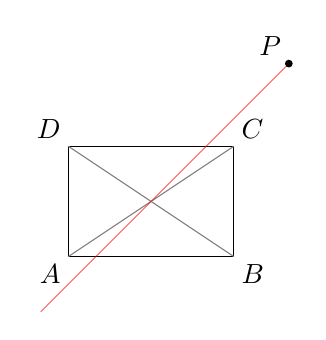
\begin{tikzpicture}[scale=0.7]
\tkzDefPoints{0/0/A, 3/0/B, 3/2/C, 0/2/D, 4/3.5/P}

\foreach \point [count = \n, evaluate = \n as \rot using
  {{-135,-45,45,135,135}[\n - 1]}] in {A,B,C,D,P}{
    %\fill (\point) circle (2pt);
    \node[label={[label distance=-6pt]\rot:$\point$}] at (\point) {};
  }

\draw (A) rectangle (C);

\tkzDrawSegments[gray, thin](A,C B,D)
%\draw[red] (1.5,1) -- (4,4);

% hi ^.^
% ok here's what to do :yaw:

\tkzDefMidPoint(A,C) \tkzGetPoint{M}
\tkzDrawLine[red,add=0 and 0.8](P,M)
\fill (P) circle (2pt);
\end{tikzpicture}

% Circle center
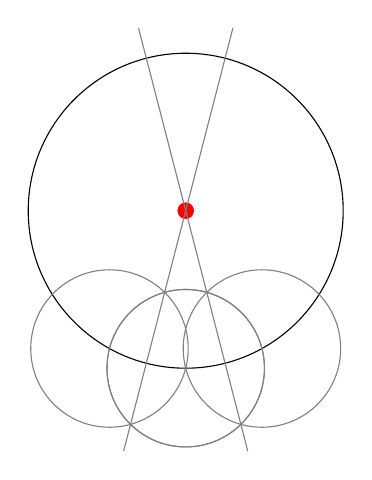
\begin{tikzpicture}[scale=2]
\tkzDefPoints{0/0/O, 0/-1/A}

\draw (O) circle (1);
  \foreach \point [count = \n, evaluate = \n as \rot using
  {{90}[\n - 1]}] in {O}{
    \fill[red] (\point) circle (1.5pt);
    %\node[label={[label distance=-4pt]\rot:$\point$}] at (\point) {};
  }
  
  \tkzInterCC[R](A, 0.5)(O, 1) \tkzGetPoints{B}{C}
  \tkzDrawCircles[gray,thin](A,B B,A A,C C,A)
  
  \tkzInterCC(A,B)(B,A) \tkzGetPoints{X1}{X2}
  \tkzInterCC(A,C)(C,A) \tkzGetPoints{Y1}{Y2}
  
  \tkzDrawLines[gray,thin,add=0.2 and 2](X1,X2 Y2,Y1)
\end{tikzpicture}
\end{document}
